\documentclass[11pt]{article}

\usepackage[a4paper,margin=1in]{geometry}
\usepackage[T1]{fontenc}
\usepackage[utf8]{inputenc}
\usepackage{lmodern}
\usepackage{setspace}
\usepackage{amsmath,amssymb}
\usepackage{booktabs}
\usepackage{multirow}
\usepackage{siunitx}
\usepackage{hyperref}
\usepackage{graphicx}
\usepackage{xcolor}
\usepackage[section]{placeins}  % prevent floats from drifting past section boundaries
\usepackage{float}              % provides [H] placement
\usepackage{flafter}            % do not place floats before their definitions

\hypersetup{
  colorlinks=true,
  linkcolor=blue!50!black,
  citecolor=blue!50!black,
  urlcolor=blue!50!black
}

\title{Learning Region-Specific Copulas from\\Marginal Constraints via Distribution-Level Diffusion}


\date{}

\begin{document}
\maketitle
\onehalfspacing

\begin{abstract}
Population synthesis from aggregate constraints requires recovering how demographic attributes co-occur within each region, not just how common each attribute is marginally. Existing methods can match target marginals, but they usually rely on shared seed distributions or other low-dimensional summaries that leave region-specific dependence weakly identified. We address this problem by training a conditional diffusion model directly on regional joint probability vectors, treating each observed region as one training example and conditioning generation on low-dimensional census summaries. We find that regional dependence is strongly heterogeneous across the United States and that the proposed model consistently improves reconstruction accuracy over a global-seed IPF benchmark, with the advantage remaining stable under held-out geographic validation. Controlled ablations further show that pairwise cross-tabulations contribute substantially more than one-dimensional marginals alone, identifying constraint informativeness rather than model capacity alone as the main driver of dependence recovery. These results show distribution-level diffusion as a practical route to learning region-specific copulas from aggregate constraints and suggest that future progress will depend more on richer conditioning statistics than on larger generative models.
\end{abstract}

%% ====================================================================
\section{Introduction}
\label{sec:intro}

The creation of a synthetic population by reconstructing the joint distribution of demographic attributes within regions from aggregated data (i.e., data reporting regional marginal distributions of individual attributes) has long been regarded as a foundation of urban simulation, transportation modeling, and policy analysis \cite{mueller2011,barthelemy2013,la2025,chapuis2022}. However, aggregated data drastically under-specify the full picture from a statistical perspective. For example, when creating a synthetic population with five attributes and four values per attribute, the joint distribution contains more than one thousand potential combinations, whereas current methods typically rely on one-dimensional marginals alone. As a result, the underlying dependence structure---that is, the copula \cite{sklar1959} describing how multiple attributes co-occur---may be missed. The resulting synthetic population can therefore contain internal bias, such as assigning an impossible combination of attributes to a single synthetic individual.

Recovering a joint distribution from marginals alone is inherently difficult because the copula is hard to reconstruct \cite{frogner2019}. Existing population-synthesis methods nevertheless attempt to address this problem through two broad strategies: synthetic reconstruction and combinatorial optimization \cite{chapuis2022}. In the synthetic-reconstruction family, methods such as Hierarchical Sampling (HS) \cite{jiang_large-scale_2024}, Iterative Proportional Fitting (IPF) \cite{predhumeau_synthetic_2023}, and Iterative Proportional Updating (IPU) \cite{ipu2009} recover joint distributions from aggregated data (e.g., census-tract-level data) by matching target marginals while preserving the seed copula structure \cite{choupani2016,lovelace2015}. In the combinatorial-optimization family \cite{harland2012}, one extends real individual-level microdata or adjusts existing synthetic individuals to match target joint distributions through fitness evaluation and optimized sampling procedures.

However, these methods share a common limitation: the copula structure is extracted from aggregated data or real individual-level microdata and then applied uniformly across regions. This works when regions are demographically similar, but when regions are heterogeneous, a fixed copula can misrepresent local dependence and introduce internal bias into the resulting synthetic population \cite{roxburgh2025}. A related issue is spatial non-stationarity \cite{krupskii2018,mondal2024,bastin2023}, which fails to reconstruct the distribution of spatial heterogeneity related to the different combinations of demographic attributes. For example, a university region with a distinctive ``young + low-income + high-education'' composition pattern does not share the same age--income--education dependence pattern as a manufacturing region. To demonstrate this spatial heterogeneity, we extract regional dependence structures across the 2,456 Public Use Microdata Areas (PUMAs) in the United States and compare each region with the national average. The mean total variation distance (TVD) is 0.19, which is far from negligible and far from uniform across regions (Figure~\ref{fig:heterogeneity}).

\begin{figure}[!bhtp]
\centering
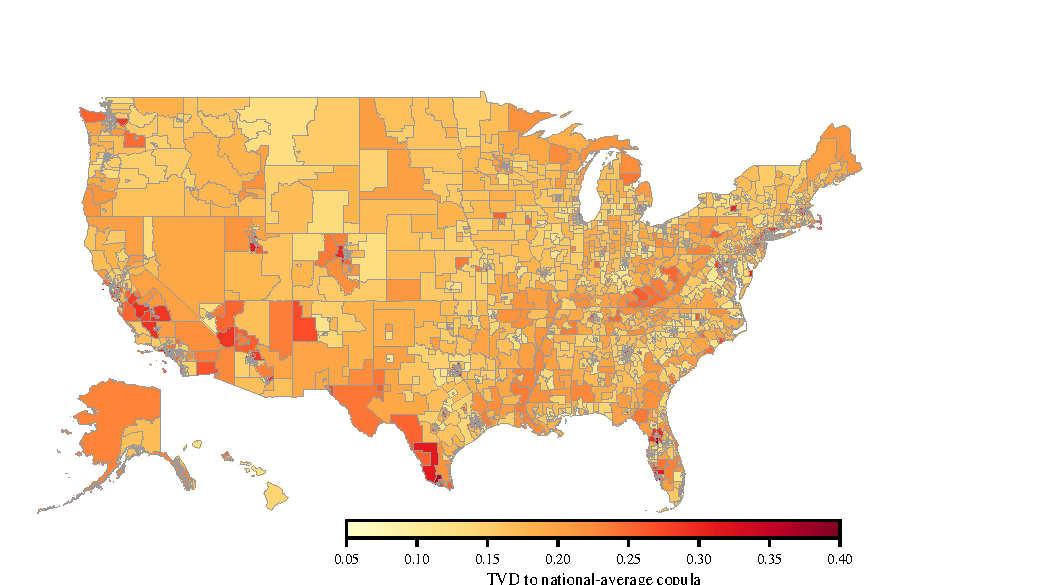
\includegraphics[width=\textwidth]{figures/fig_01_map.pdf}
\caption{Spatial heterogeneity of dependence structure across regions in the United States.
Choropleth of PUMA-level TVD to the national-average joint distribution ($K=32$, five demographic attributes). Michigan, the held-out test state used in later regional validation, is outlined in blue.}
\label{fig:heterogeneity}
\end{figure}

To handle such copula structures, optimization methods such as integer least squares programming have been used to create synthetic populations for the United States from Census Block Group data \cite{lin2023}. Parametric approaches instead use statistical inference to learn the joint relationship among hidden attributes in the data. Examples include methods based on Markov Chain Monte Carlo \cite{farooq2013} and Bayesian-network sampling \cite{zhou_creating_2022}. A persistent limitation, however, is that the resulting spatial non-stationarity remains unresolved because the same set of parameters or the same structural template is used throughout the synthesis process.

Recently, generative models have provided a new possibility for recovering the correct copula structure while addressing spatial non-stationarity in synthetic populations \cite{sane2025}. Among them, diffusion models are particularly well suited to this task because they can learn the joint distribution through an iterative denoising process, without requiring a predefined copula template or hand-specified parameter settings \cite{ho2020}. Conditional diffusion is especially relevant because it can use regional demographic summaries as constraints while allowing the dependence structure itself to vary across space. 

The goal of this work is to propose a generative framework using a diffusion model to generate the synthetic population. 

In this paper, we therefore ask whether a diffusion model trained on PUMA-level distributions can recover region-specific copulas more accurately than methods that rely on a single national seed.

Although the generative problem is defined at the PUMA level, the recovered regional full joint is ultimately used to construct point-level spatial synthetic population data.





%The field has developed effective solutions to this problem, each under specific conditions. IPF-based reweighting \cite{deming1940,bishop1975,choupani2016,lovelace2015} recovers accurate joints when a representative seed table is available: IPF adjusts the seed to match target marginals while preserving the seed's dependence structure \cite{csiszar1975}. Combinatorial optimization \cite{harland2012} can match target distributions when the candidate microdata pool covers the target support. Bayesian network sampling \cite{farooq2013} and integrated frameworks such as simPop \cite{templ2017} succeed when a correct parametric or structural prior can be specified.

%In practice, however, per-record training losses optimize marginal accuracy far more efficiently than dependence accuracy. The reason is structural: if 80\% of a region's residents are young, then 80\% of training records contain ``young''---the marginal frequency is directly encoded in the data frequency, producing a strong, consistent gradient. Dependence, by contrast, concerns the relative frequency of attribute combinations: a single training record (young, low-income) is equally consistent with $P(\text{low-income}\mid\text{young})=0.8$ and $P(\text{low-income}\mid\text{young})=0.7$---both copulas frequently produce this record, so per-record losses cannot distinguish between them. The gradient signal for dependence is therefore weak and noisy. We confirmed this empirically: a person-level conditional diffusion model, even with exact region identity as input, produced copula TVD of 0.159 across Michigan's 68 regions---systematically worse than the 0.137 obtained by na\"ively reusing the training-region average (Supplementary Fig.~S1).

%---a form of spatial non-stationarity well recognized in the copula literature \cite{krupskii2018,mondal2024,bastin2023}. Moving beyond the direct reweighting or resampling of existing records, statistical inference is another approach to dealing with such issue 
%The direct route eliminates this signal asymmetry.We train a conditional denoising diffusion model to predict the regional joint probability vector---a single vector whose entries encode both marginal frequencies and their couplings. 

%In this formulation, copula errors are immediately visible in the loss function and optimized with the same directness as marginal errors. Each of 2,456 observed regional distributions becomes one training example, and the model learns to map marginal (and optionally pairwise) constraints to the full joint \cite{floto2023,avdeyev2023}. In practice, the diffusion model produces a region-specific joint distribution from marginal inputs; one round of IPF then enforces exact marginal consistency, and standard sampling yields individual synthetic records. The IPF baseline follows the same post-processing but starts from a national-average joint distribution, so the comparison isolates how well each approach captures region-specific dependence (Fig.~\ref{fig:schematic}).Distribution-level diffusion consistently outperforms global-seed IPF across all five tested configurations with up to 256 joint cells, achieving up to 59\% error reduction. A five-fold spatial cross-validation on held-out regions confirms statistical significance ($p = 0.031$). Systematic ablations reveal that the critical determinant of performance is not model architecture but the informativeness of input constraints: two-variable cross-tabulations provide up to 44\% additional improvement over one-variable summaries alone.

%% ====================================================================

% start to revise the result
\FloatBarrier
\section{Methods}

\subsection{Overview}
As discussed in Section~\ref{sec:intro}, our goal is to recover joint distributions over age, sex, education, employment, and income for individual PUMAs from external census summaries and convert them into point-level spatial synthetic population data. The framework comprises three steps, summarized in Figure~\ref{fig:framework}. First, for each of the 2,456 Public Use Microdata Areas (PUMAs) in the United States, Step~1 constructs training targets extracted from PUMS microdata and aligns them with external census summaries. Second, Step~2 learns hierarchical joint distributions from these external census summaries through two sub-stages. Within Step~2, Stage~1 predicts a coarse regional distribution, and Stage~2 refines it into the joint distribution over the five variables for each PUMA. Third, Step~3 samples synthetic persons from the learned joint distribution and assigns explicit home and work locations using tract-level ACS summaries, road-network data, and commuting-flow data derived from LODES. This produces point-level spatial synthetic population data.


\begin{figure}[H]
\centering
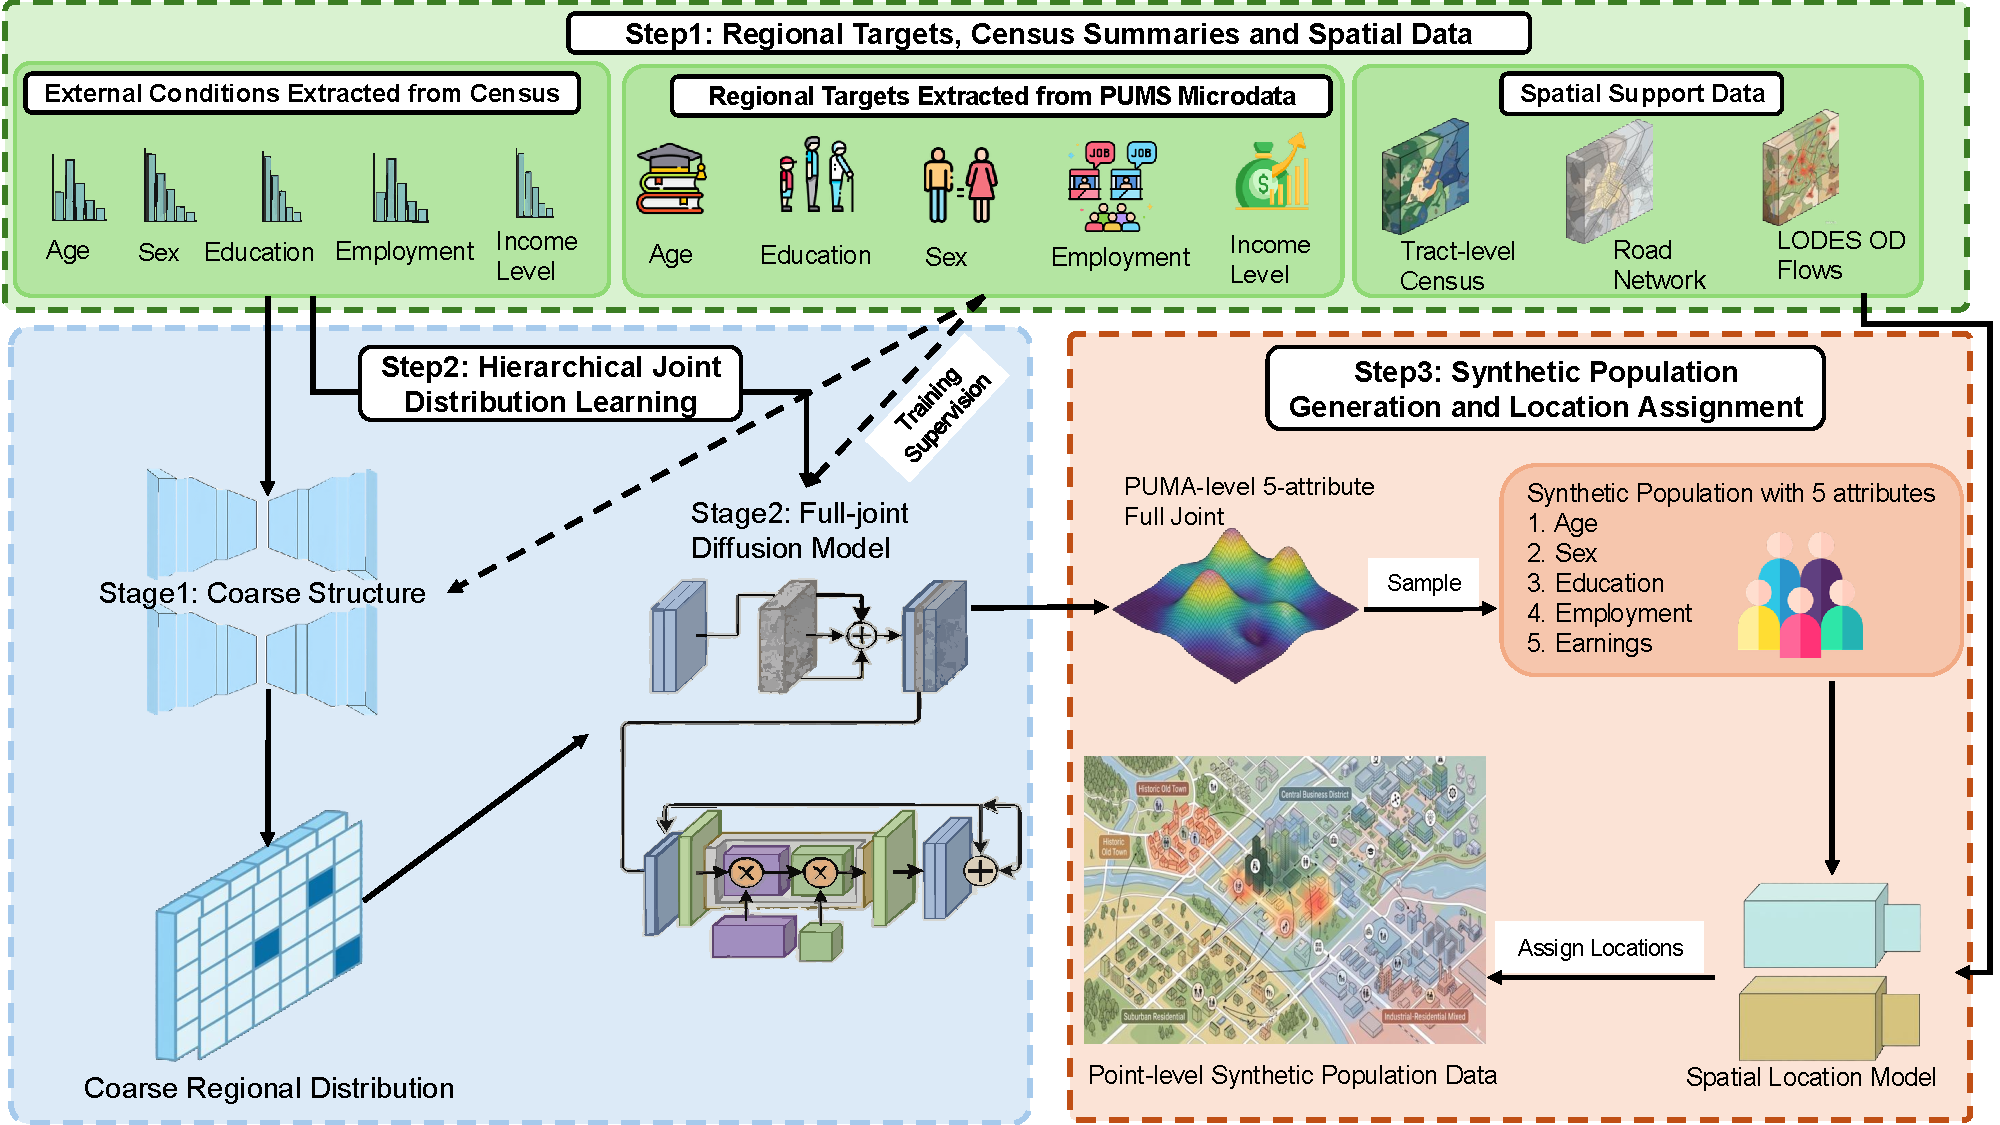
\includegraphics[width=\textwidth]{figures/fig_02_framework.pdf}
\caption{Framework for hierarchical generation of joint distributions for PUMAs and point-level location assignment for synthetic populations.}
\label{fig:framework}
\end{figure}



\subsection{Data Sources}\label{sec:data_sources}

As shown in Figure~\ref{fig:framework}, the framework requires three kinds of data: regional training targets, external condition inputs, and spatial data for explicit location assignment. Table~\ref{tab:data} summarizes the corresponding sources and their roles in the framework.

\begin{table}[!bhtp]
\centering
\small
\caption{Data sources used in the main framework.}
\label{tab:data}
\begin{tabular}{p{0.20\linewidth}p{0.23\linewidth}p{0.16\linewidth}p{0.33\linewidth}}
\toprule
Data type & Source & Scale & Role in framework \\
\midrule
Regional training targets & 2023 five-year ACS Public Use Microdata Sample (PUMS) \cite{acs,pums} & Person-level microdata aggregated to PUMA & Construct region-specific training targets defined as joint distributions for individual PUMAs \\
External condition inputs & Published ACS summary tables \cite{acs} & PUMA-level summaries & Derive external census summaries used during training and inference in Step~2 \\
Spatial data for location assignment & Tract-level ACS summaries \cite{acs}, OpenStreetMap road network \cite{openstreetmap}, and LODES commuting flows \cite{lodes} & Tract, road segment, and tract-to-tract flow & Support tract allocation and explicit home/work location assignment in Step~3 \\
\bottomrule
\end{tabular}
\end{table}

The first data source is the 2023 five-year American Community Survey (i.e., ACS) Public Use Microdata Sample (i.e., PUMS), covering 2,456 Public Use Microdata Areas (PUMAs) in the United States \cite{acs,pums}. We use PUMS to construct region-specific training targets. The rationale is that PUMS is an individual-level sample representing approximately 5\% of the population, so each PUMA can be represented by an empirical regional joint distribution that preserves copula structure and spatial heterogeneity more faithfully than marginal frequencies alone.

The second data source is the published ACS summary tables at the PUMA level \cite{acs}. We use these tables to derive the external census summaries that condition the framework during both training and inference in Step~2. The rationale is that the ACS tables contain the standard census variables available for unseen regions, but only limited cross-variable information. Learning the mapping from these external census summaries to the PUMS-derived regional targets is therefore the central inference problem addressed in Step~2.

The third data source comprises the spatial data used in Step~3 to convert the generated regional joint distribution into explicit point-level locations. These data include tract-level ACS summaries \cite{acs}, road-network data from OpenStreetMap \cite{openstreetmap}, and commuting-flow data derived from LODES \cite{lodes}. Tract-level ACS summaries anchor tract-level residential allocation, road-network data support explicit point placement, and commuting-flow data provide the destination-tract structure needed for workplace assignment. Across the framework, the final synthetic population is defined on five person-level attributes: age, sex, education, employment, and income. 
\subsection{Step 1: Constructing PUMA-Level Targets and External Census Summaries}
\label{sec:training_target}
As shown in Figure~\ref{fig:framework}, Step~1 constructs two aligned vectors for each PUMA. One is a training target $\mathbf{p}$, defined as the joint distribution over the five variables for that PUMA. The other is a condition vector $\mathbf{c}$, derived from the external census summaries. Across the United States, this yields 2,456 aligned $(\mathbf{c}, \mathbf{p})$ pairs for Step~2.

To construct $\mathbf{p}$, we first align the PUMS variables to the standard census variables summarized in Table~\ref{tab:var_attr}. Age is discretized into census-aligned bins. Education and employment retain all-population coverage by assigning people not covered by the corresponding ACS tables to explicit residual categories. Income is represented with six groups, and people younger than 16 or with no reported earnings are also assigned to a residual category. This preprocessing ensures that the regional targets and the external census summaries are defined on the same five-variable state space.

On this aligned state space, we construct the target vector $\mathbf{p}$ from cell counts over the five variables using survey weights. Each cell records the probability of one age--sex--education--employment--income combination within a PUMA. To avoid zero-probability cells in sparse regional tables, we add a Laplace pseudo-count ($\alpha=1$) to each cell and then normalize the table to sum to one. The resulting vector $\mathbf{p}$ is the empirical joint distribution over the five variables for that PUMA and serves as the regional target in Step~2.

For the same PUMA, we construct the condition vector $\mathbf{c}$ by concatenating the normalized ACS summaries for age, sex, education, employment, and income. Each summary is normalized within variable, so $\mathbf{c}$ represents the regional marginal distributions of the five variables rather than raw population size. Like $\mathbf{p}$, $\mathbf{c}$ is defined on the same PUMA geography and the same five-variable state space. The two vectors play different roles. $\mathbf{p}$ provides the supervision target. $\mathbf{c}$ provides the observable conditioning input.

\begin{table}[!bhtp]
\centering
\small
\caption{Operational variables and ACS--PUMS alignment for the joint distribution over the five variables in each PUMA used in the main framework.}
\label{tab:var_attr}
\begin{tabular}{p{0.11\linewidth}p{0.13\linewidth}p{0.14\linewidth}p{0.24\linewidth}p{0.28\linewidth}}
\toprule
Variable & ACS Source & PUMS Variable & Format & Description \\
\midrule
Age & B01001 & AGEP & Census-aligned age bins & Fine-grained age groups used in the regional state space. \\
Sex & B01001 & SEX & Binary sex categories & Directly aligned across ACS and PUMS. \\
Education & B15003 & SCHL & All-population categories with an explicit residual category & Includes an explicit category for people not covered by the ACS education table. \\
Employment & B23025 & ESR & All-population categories with an explicit residual category & Includes an explicit category for people not covered by the ACS employment table. \\
Income & B20001 & PERNP & Six income categories aligned with PUMS variable PERNP, plus a residual category & People younger than 16 or with no reported earnings are assigned to the residual category. \\
\bottomrule
\end{tabular}
\end{table}

\subsection{Step 2: Learning Hierarchical Joint Distributions}
\label{sec:training_model}
As shown in Figure~\ref{fig:framework}, Step~2 learns a mapping from the external census summaries to the joint distribution over the five variables for each PUMA. This is difficult because the census summaries contain the regional distribution of age, sex, education, employment, and income, but not how the five variables co-occur jointly within each PUMA. We therefore decompose Step~2 into two sub-stages. Stage~1 predicts a coarse regional distribution, and Stage~2 refines that coarse structure into the joint distribution used in Step~3.

Before training Stage~1 and Stage~2, we transform the target vector $\mathbf{p}$ into a more stable continuous representation by mapping it to log-probability space.
\[
  \mathbf{x}_0 = \log(\mathbf{p}+\phi), \quad \phi=10^{-6},
\]
This reduces the gap between common and rare cells and makes the diffusion target numerically more stable. We then standardize the transformed vectors within each training split.
\[
  \mathbf{z}_0 = \frac{\mathbf{x}_0 - \boldsymbol{\mu}_{\text{train}}}{\boldsymbol{\sigma}_{\text{train}}},
\]
where $\boldsymbol{\mu}_{\text{train}}$ and $\boldsymbol{\sigma}_{\text{train}}$ are computed from that split only. A floor of $10^{-6}$ is applied to $\boldsymbol{\sigma}_{\text{train}}$ for numerical stability.

In Stage~1, we construct a coarser version of the regional joint distribution by merging the original groups for age, education, employment, and income. Sex remains binary. Age is reduced from 10 bins to 4, education from 5 groups to 3, employment from 5 groups to 3, and income from 6 groups to 4. This yields a $4 \times 2 \times 3 \times 3 \times 4$ coarse joint with 288 cells. Stage~1 then predicts this coarse distribution from the external census summaries. We select the model using validation TVD on this coarse target.

In Stage~2, the model determines how the probability in each coarse group should be split across the finer variable combinations nested within that group. The main estimate is produced by the diffusion path through denoising, which refines the coarse regional structure into the joint distribution over the five variables.

During training, Stage~2 receives two forms of coarse input. One is the true coarse version of the PUMS-derived regional joint distribution. The other is the coarse prediction produced by Stage~1. This exposes Stage~2 both to the true coarse distribution and to the Stage~1 prediction it will receive in the full pipeline. The two sub-stages therefore reconstruct the joint distribution used in Step~3.

\subsection{Step 3: Synthetic Population Generation and Location Assignment}
\label{sec:inference}

As shown in Figure~\ref{fig:framework}, Step~3 converts the reconstructed joint distribution for each PUMA into point-level spatial synthetic population data. This step first samples synthetic persons from that joint distribution and then assigns explicit home and work locations using the spatial data introduced above.

For each PUMA, we first sample synthetic persons from the predicted joint distribution over the five variables so that the sampled population matches the survey-weighted PUMA population total used to construct the target vector $\mathbf{p}$ in Step~1. After this sampling step, each synthetic person already carries age, sex, education, employment, and income. The remaining task is to assign spatial locations.

We next use the tract-level ACS summaries, road-network data, and commuting-flow data derived from LODES introduced in Section~\ref{sec:data_sources} to assign these locations. Tract-level ACS summaries allocate sampled residents across tracts within each PUMA, and road-network data place explicit home points within the assigned tracts. For workers, commuting-flow data derived from LODES first assign work destination tracts. Road-network data then place explicit work points within those tracts. The output of Step~3 is therefore a point-level spatial synthetic population in which each person retains the five person-level attributes together with an explicit home location, and workers are additionally assigned explicit work locations. 

\subsection{Regional Validation and Baseline Comparison}
\label{sec:experiment}

After Step~2 reconstructs the joint distribution over the five variables for each PUMA, we evaluate how accurately this regional distribution is recovered on Michigan's 68 PUMAs excluded from training. Michigan spans metropolitan, suburban, and rural contexts, and its heterogeneity lies within the national range rather than forming an extreme outlier (Figure~\ref{fig:heterogeneity}; Supplementary Figure~\ref{fig:S2_heterogeneity}). This setting therefore tests whether the model recovers region-specific dependence in geographies excluded from training.

We evaluate reconstruction accuracy with total variation distance (TVD) \cite{lovelace2015},
\[
  \text{TVD} = \frac{1}{2}\sum_k|\hat{p}_k-p_k| ,
\]
where $\hat{\mathbf{p}}$ denotes the predicted joint distribution over the five variables and $\mathbf{p}$ denotes the observed PUMS-derived target for a given PUMA. Lower TVD indicates closer agreement between the predicted and observed regional joint distributions.

In this Michigan evaluation, the main quantity is the TVD of the hierarchical model when Stage~1 and Stage~2 are run together. We compare the hierarchical model with two alternatives. The first is a one-shot diffusion model that predicts the joint distribution directly from the external census summaries, without coarse-to-fine decomposition. The second is IPF, which uses the same observed five-variable marginals as a reference baseline. We also report one diagnostic variant in which Stage~2 receives the true coarse regional distribution instead of the Stage~1 prediction. All main quantitative results are reported over three random seeds as mean $\pm$ standard deviation.

The preceding protocol evaluates only recovery of the regional joint distribution. We evaluate the spatial assignment in Step~3 separately in metropolitan Detroit with external mobility data, which provide independent residential and workplace references for the spatial product. For the home layer, we compare tract-level residential shares with Spearman correlation, cosine similarity, and TVD, and we further evaluate within-tract residential ordering with block-group-level rank comparisons. For the work layer, we compare destination-tract workplace shares with the same tract-level metrics and evaluate commute-distance distributions with cosine similarity and TVD.

%% ====================================================================
\section{Results}
\subsection{Spatial Population Generation}

This subsection establishes the form of the final spatial product. The generated population is represented as a point-level spatial synthetic population. Each sampled person retains the five person-level attributes and is assigned an explicit home location, while workers are additionally assigned work locations. Figure~\ref{fig:detroit_overview} illustrates this product in metropolitan Detroit.

Panels a--c of Figure~\ref{fig:detroit_overview} show that the residential layer is spread across the metropolitan region, with the highest density in the southeastern urban core. This residential distribution remains relatively broad, with the top 10\% of tracts containing 18.1\% of residents. Panels d--f show a much more concentrated work layer, with workplace destinations clustered in a smaller set of tracts and the sampled work points forming a sharper spatial core. In this work layer, the top 10\% of tracts contain 50.4\% of workplace destinations. Figure~\ref{fig:detroit_overview} therefore shows a product in which residential population is distributed across many tracts, while workplace destinations are concentrated much more strongly.

\begin{figure}[!bhtp]
\centering
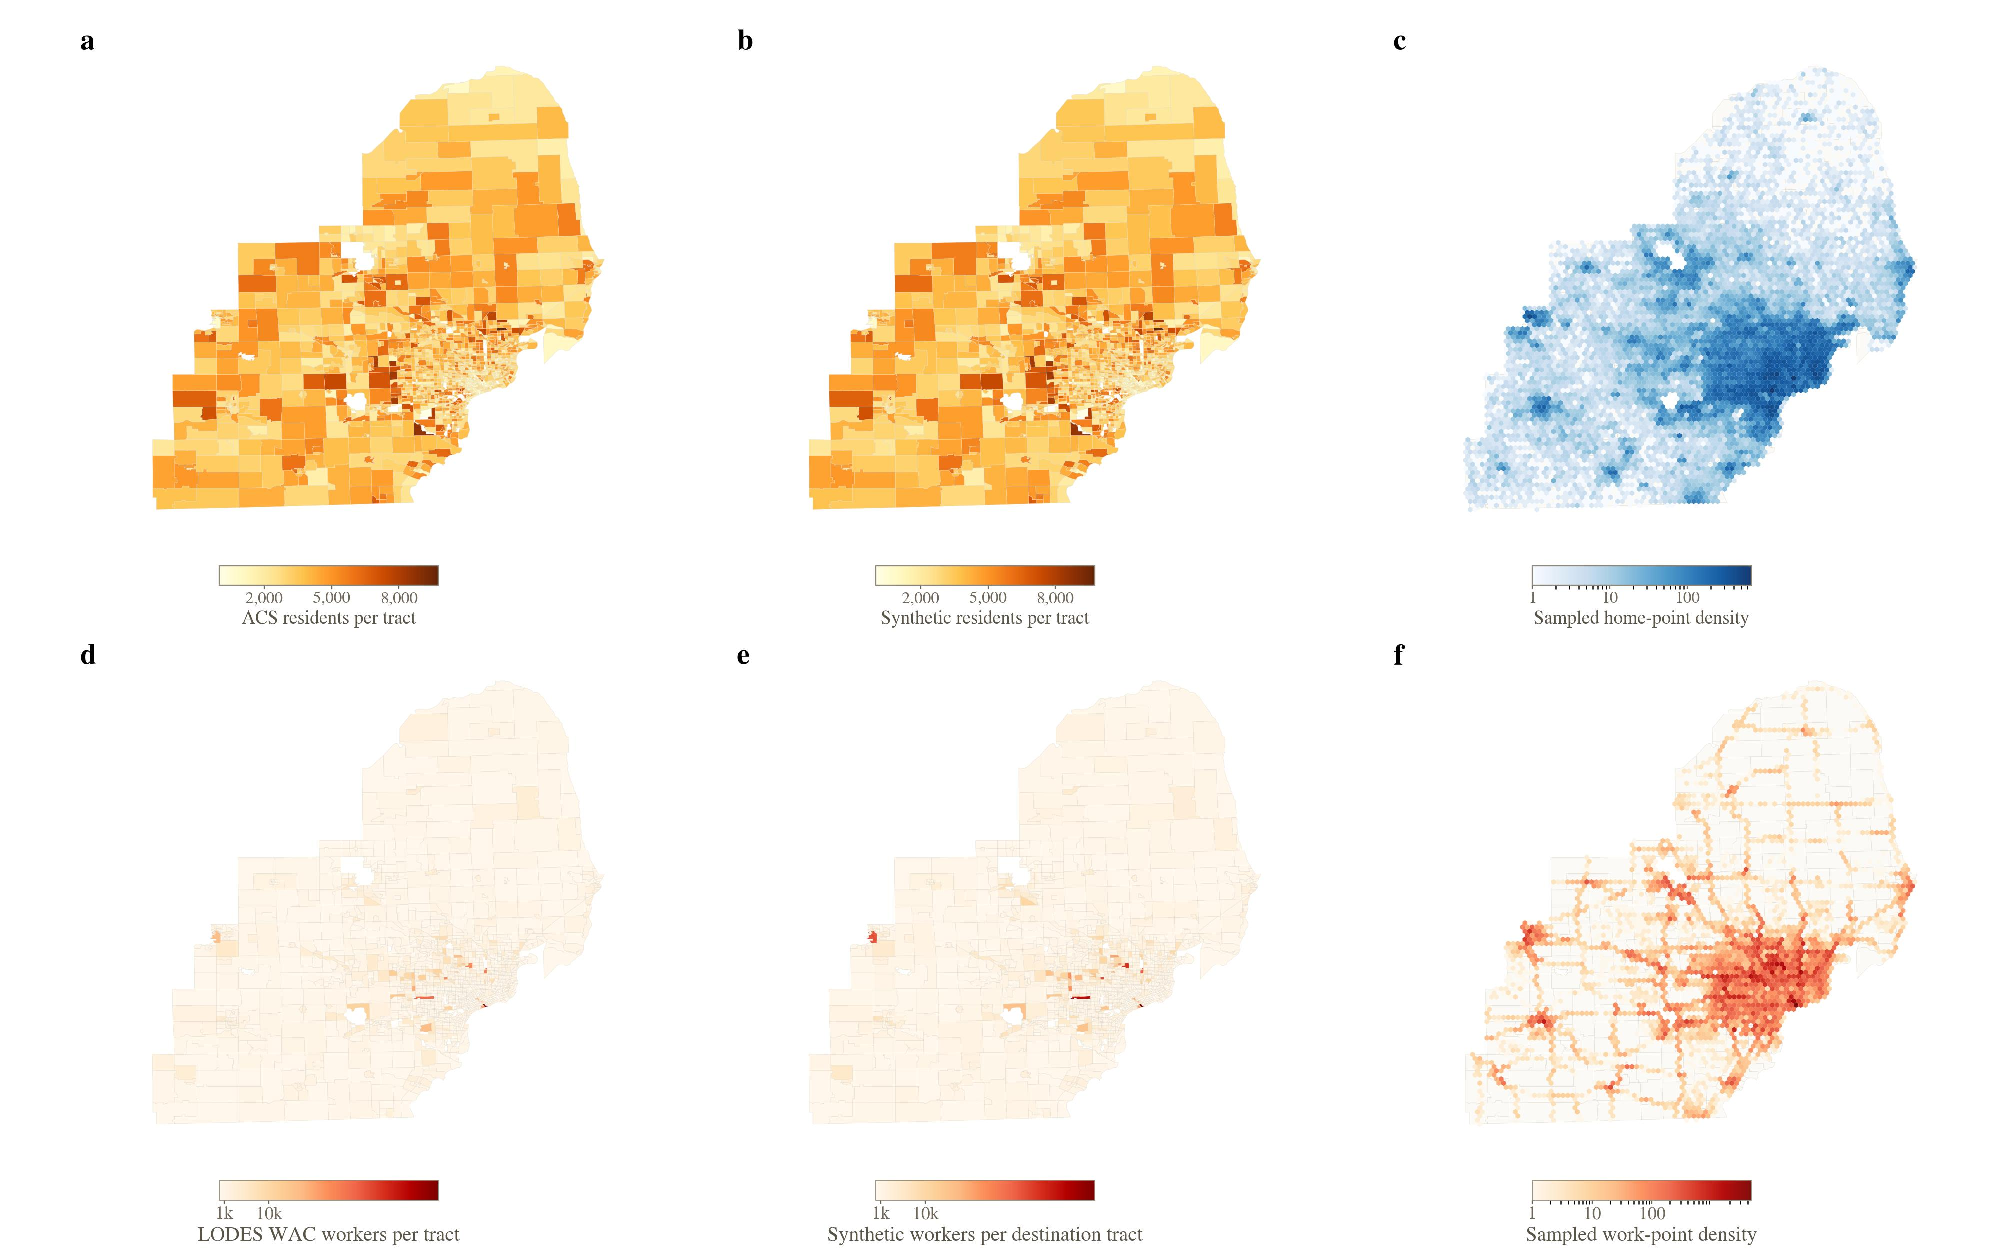
\includegraphics[width=\textwidth]{figures/fig_03_spatial_product_overview.pdf}
\caption{Detroit overview of the point-level spatial synthetic population. Panels a--c show the residential layer: the ACS tract-level residential reference, synthetic residents per tract, and sampled home-point density. Panels d--f show the work layer: the LODES tract-level workplace reference, synthetic workers per destination tract, and sampled work-point density.}
\label{fig:detroit_overview}
\end{figure}

The same spatial product also resolves tract-level residential composition for all five variables. Figure~\ref{fig:attribute_patterns} maps one representative slice for each variable. Panels a--c show age, sex, and employment composition. Children are spread across many tracts, female shares vary more mildly across the region, and employed shares are higher in a more limited set of tracts. Panels d and e show education and income composition, with bachelor's-plus shares and \$100k+ income shares concentrated more strongly around the metropolitan core. Figure~\ref{fig:attribute_patterns} therefore shows that the product supports attribute-conditioned spatial analysis across all five variables, not only aggregate population counts.

These subgroup patterns are also highly consistent with the corresponding tract-level ACS tables aligned to the same variables. The tract-share Spearman correlations are 0.998 for children, 0.997 for female residents, 0.935 for employed residents, 0.991 for bachelor's degree or higher, and 0.987 for income \$100k+$. Figures~\ref{fig:detroit_overview} and \ref{fig:attribute_patterns} together establish the spatial population that is evaluated in the following subsections.

\begin{figure}[!bhtp]
\centering
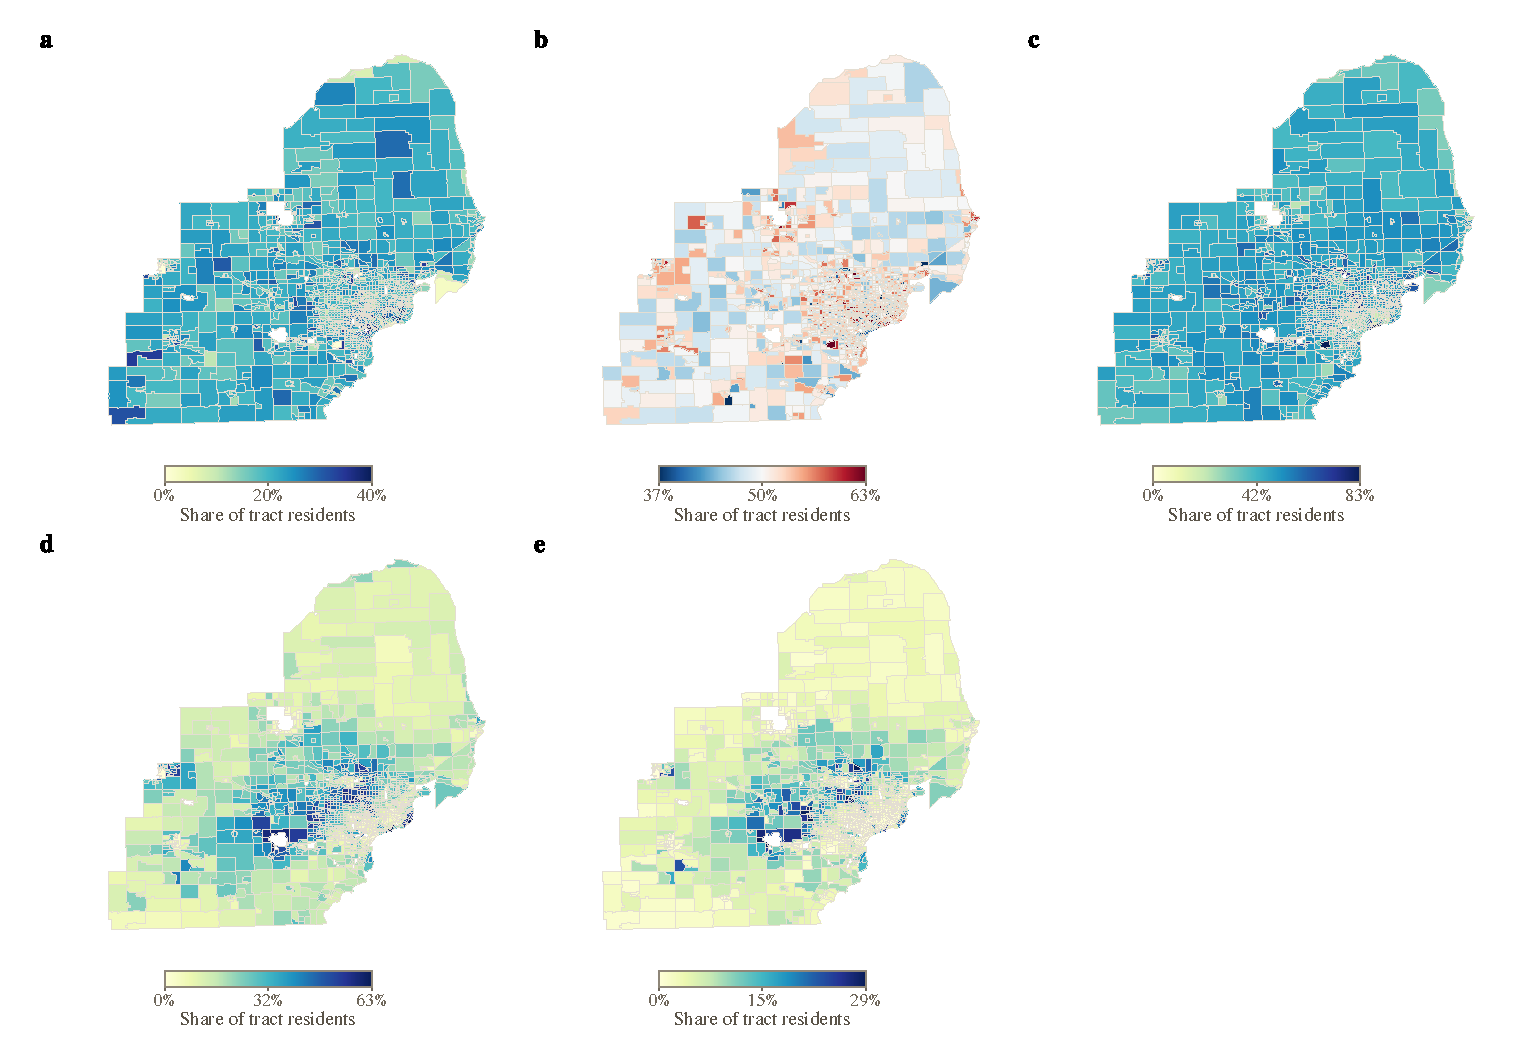
\includegraphics[width=\textwidth]{figures/fig_04_attribute_spatial_patterns.pdf}
\caption{Attribute-conditioned residential patterns in the Detroit synthetic population. Panels a--e map tract-level shares of children (ages 0--17), female residents, employed residents, residents with bachelor's degree or higher, and residents with income \$100k+, respectively. All shares are computed from the synthetic home population assigned to each tract.}
\label{fig:attribute_patterns}
\end{figure}

\FloatBarrier

\subsection{Regional Validation}
\label{sec:heldout_validation}

Figure~\ref{fig:heterogeneity} established that dependence structure varies substantially across regions. We evaluate recovery of the joint distribution on Michigan's 68 PUMAs excluded from training, before explicit location assignment. When Stage~1 and Stage~2 are run together, the hierarchical model reaches a TVD of $0.12121 \pm 0.00032$ across three seeds. This is lower than both the one-shot model, which reaches $0.14707 \pm 0.00016$, and the IPF reference baseline at $0.12698$. All three seeds of the hierarchical model also fall below the IPF baseline (0.12110, 0.12167, and 0.12107).

Figure~\ref{fig:michigan_validation} shows that this gain extends across most of Michigan. The map and per-PUMA comparisons indicate that the improvement is geographically widespread, and the ordered error curves show the same pattern across the full distribution of test PUMAs. The hierarchical model improves on IPF in 53 of 68 Michigan PUMAs. By contrast, the one-shot model does not outperform IPF in any Michigan PUMA. Panel~d shows where this advantage comes from. Each pairwise quantity is obtained by summing the joint distribution over the five variables across the other three variables and then computing TVD on the resulting two-variable distribution. The largest pairwise gains appear in education--employment, sex--employment, education--income, and age--income, while the gain for age--sex is much smaller. This pattern is consistent with the information structure of the external census summaries. Age and sex are jointly constrained by the published table B01001, whereas the other variable pairs are recovered from the learned regional dependence structure. Overall, the Michigan results show that the hierarchical model improves recovery of the regional joint distribution and that much of this advantage comes from dependencies recovered from the learned regional structure.

\begin{figure}[!bhtp]
\centering
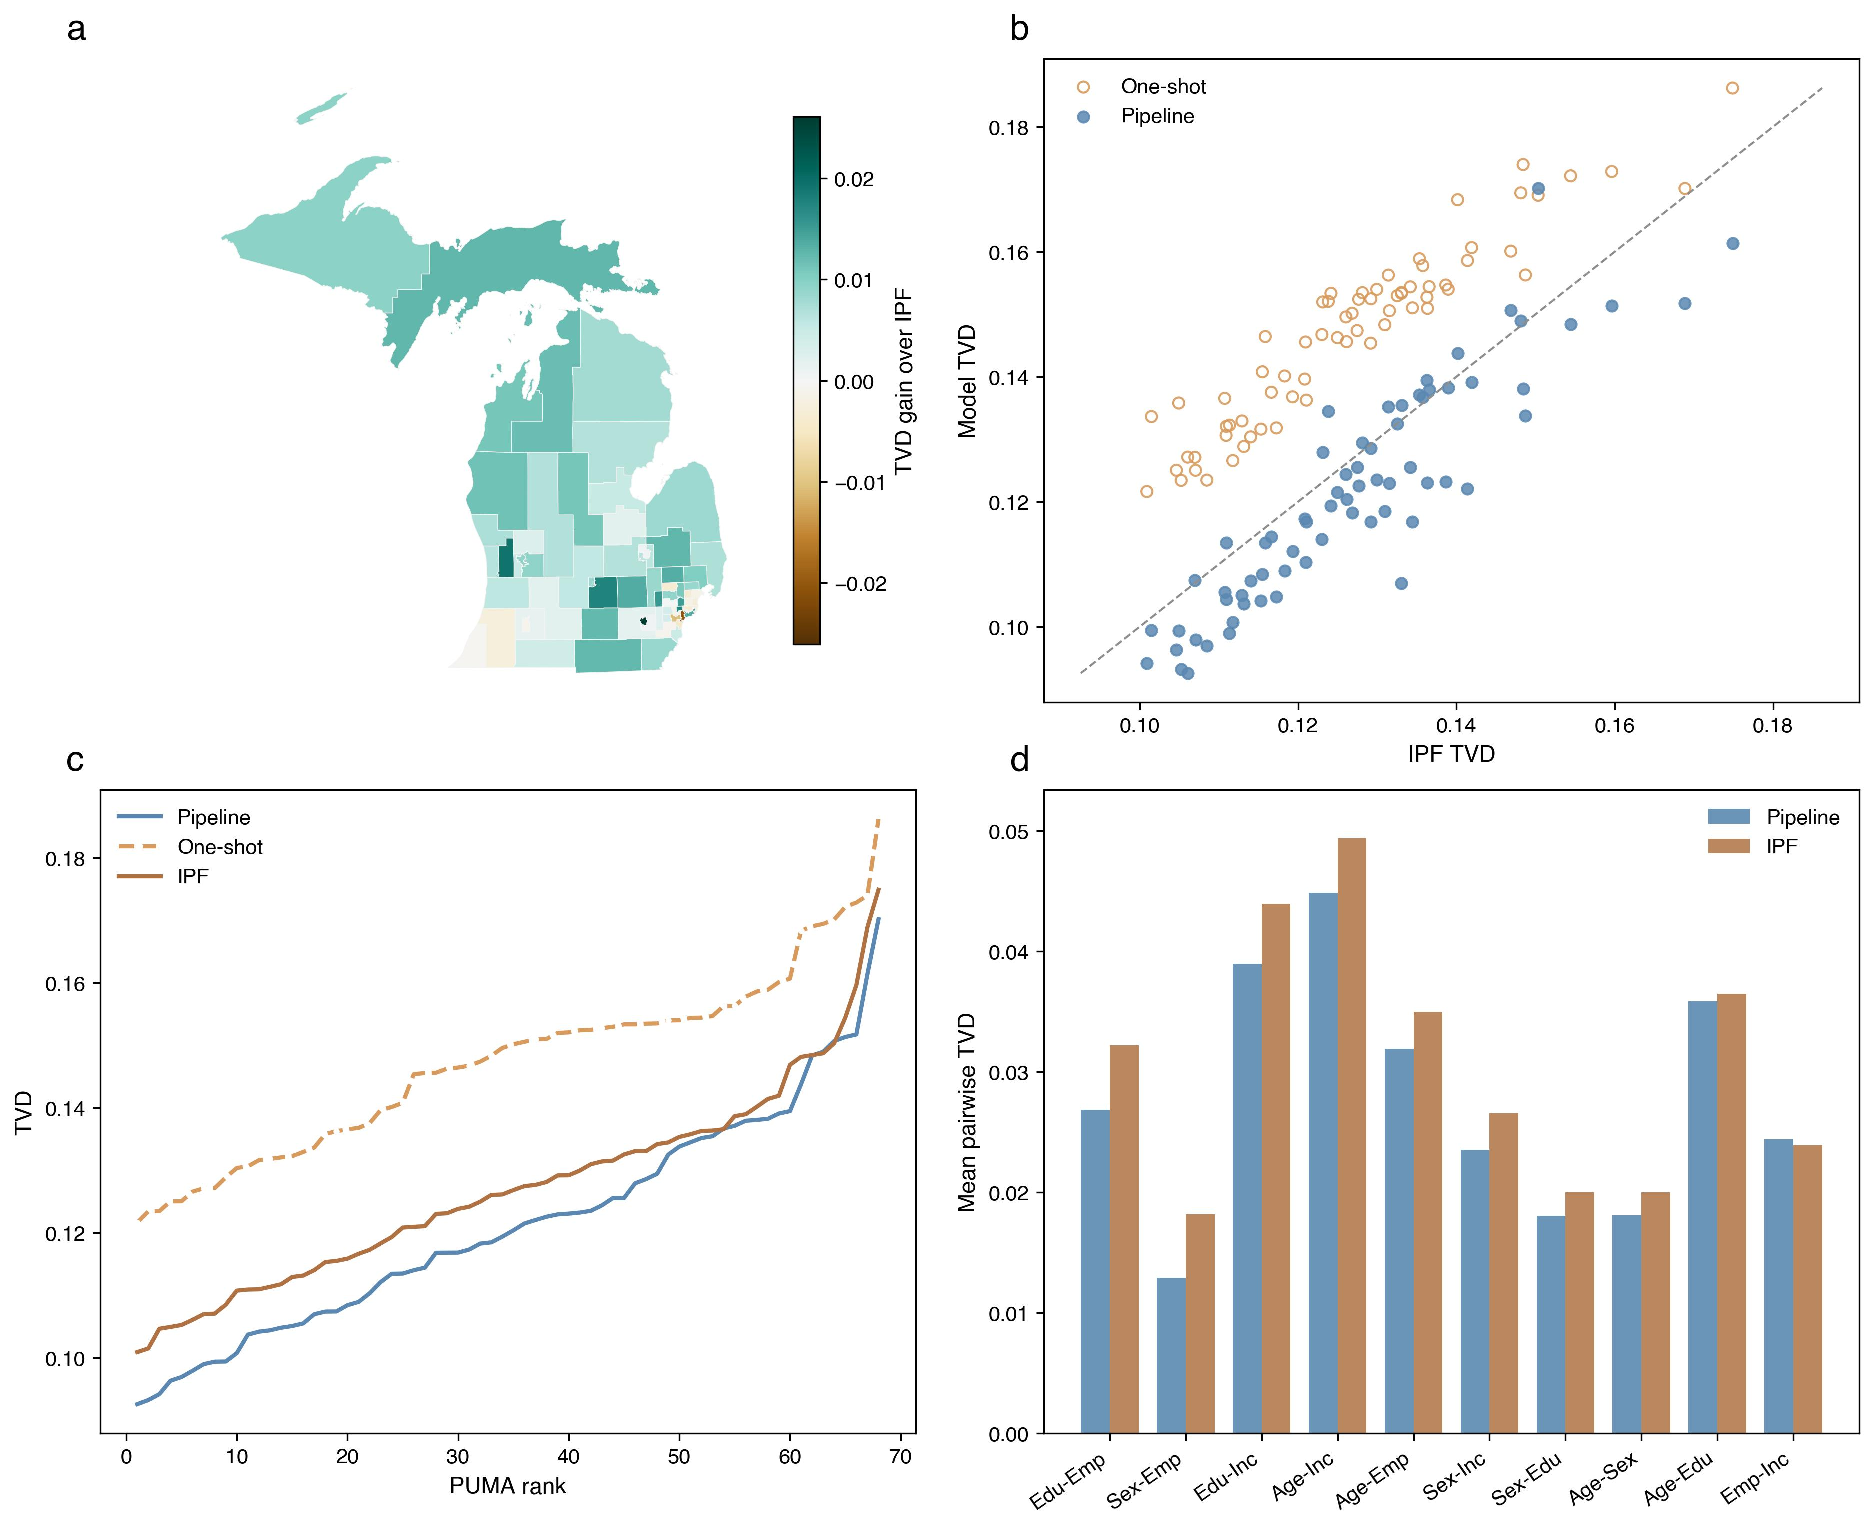
\includegraphics[width=\textwidth]{figures/fig_05_michigan_regional_validation.pdf}
\caption{Regional validation on Michigan PUMAs excluded from training. Panel a maps the per-PUMA improvement of the hierarchical model over IPF, measured as $\mathrm{TVD}_{\mathrm{IPF}} - \mathrm{TVD}_{\mathrm{hier}}$, so positive values indicate lower error for the hierarchical model. Panel b compares per-PUMA TVD against IPF for the hierarchical model and the one-shot model; points below the dashed line indicate improvement over IPF. Panel c shows ordered TVD across the 68 Michigan PUMAs for the hierarchical model, the one-shot model, and IPF. Panel d decomposes the result into the 10 variable pairs. For each pair, the joint distribution over the five variables is summed across the other three variables to obtain a two-variable distribution, and TVD is then computed on that reduced table.}
\label{fig:michigan_validation}
\end{figure}

\FloatBarrier

\subsection{External Spatial Validation}

The Michigan regional results establish the quality of the learned joint distribution. We next evaluate the explicit spatial product in metropolitan Detroit, which provides a concrete metropolitan case within the held-out Michigan setting together with independent mobility evidence for residential and workplace patterns. For this external validation, we use single-day point-level GPS stay-event data from SafeGraph, collected on 2019-02-06 within the Detroit validation area \cite{safegraph2019}. We derive nighttime residential anchors and daytime workplace anchors from these records and aggregate them into residential and workplace reference shares. Figure~\ref{fig:detroit_validation} summarizes the validation patterns discussed below. For the home layer, synthetic tract shares reach a Spearman correlation of 0.808, a cosine similarity of 0.880, and a TVD of 0.117. Within tracts, block-group ordering is positively aligned for most tracts. Among 1,515 tracts with valid block-group comparisons, the median block-group-level Spearman is 0.600 and 63.2\% of tracts exceed a threshold of 0.5. The home layer therefore captures both the broad residential geography and much of the within-tract residential ordering.

For the work layer, work-tract shares reach a Spearman correlation of 0.585, a cosine similarity of 0.823, and a TVD of 0.323 against the tract-level work reference derived from the same external mobility GPS stay-event data. The commute-distance distribution is also well matched. The synthetic median commute distance is 9.98 km, compared with a mobility median of 9.33 km, with cosine similarity 0.986 and TVD 0.090. These results show that the current work layer captures the main workplace geography and the overall commute scale.

\begin{figure}[!bhtp]
\centering
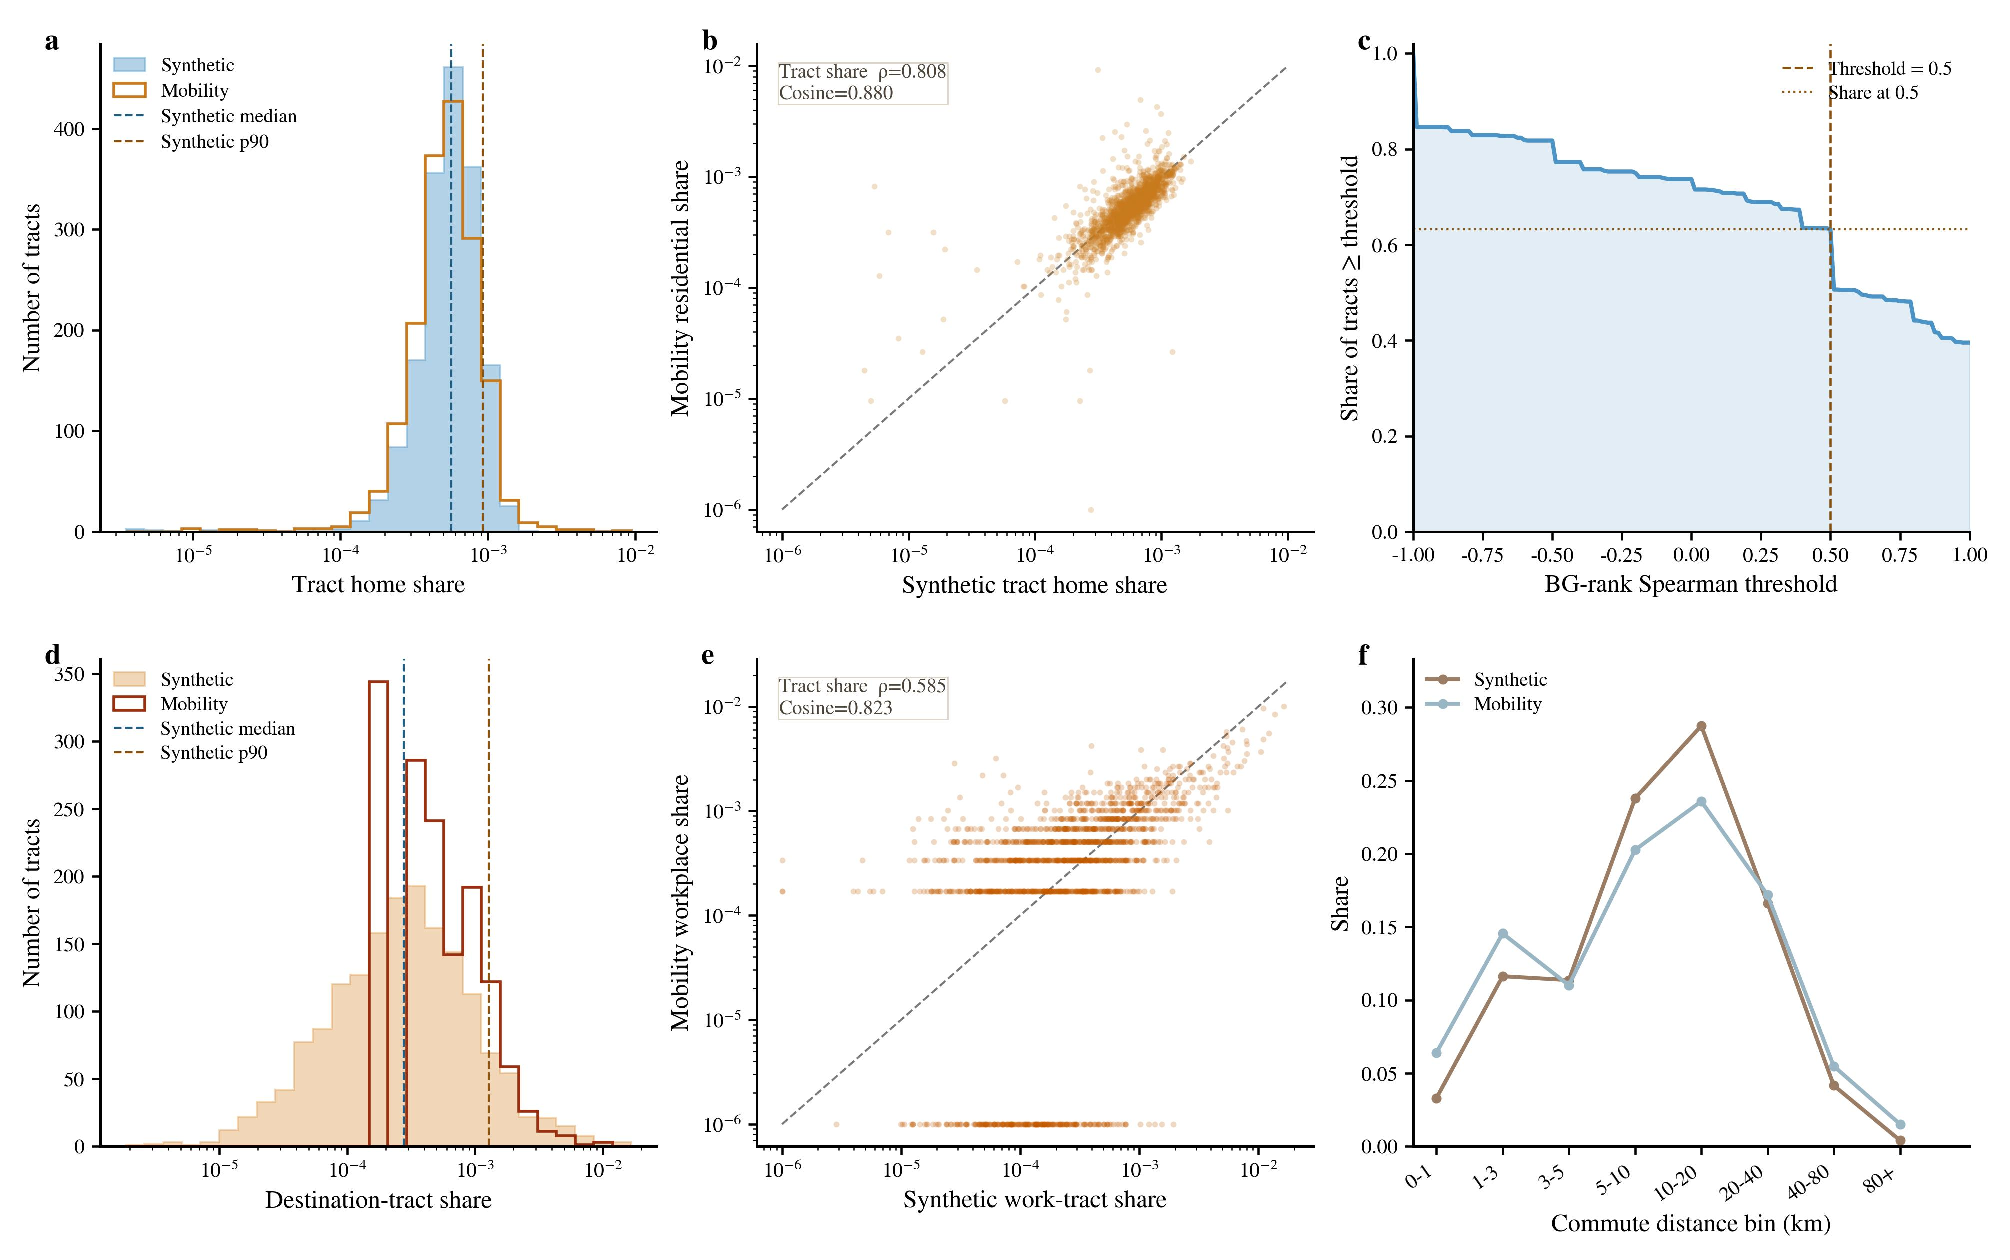
\includegraphics[width=\textwidth]{figures/fig_06_spatial_validation_overview.pdf}
\caption{External spatial validation in Detroit. Panels a--c compare synthetic and mobility-derived residential patterns through tract-share distributions, tract-level agreement, and within-tract block-group rank structure. Panels d--f compare synthetic and mobility-derived workplace patterns through destination-tract share distributions, tract-level agreement, and commute-distance distributions.}
\label{fig:detroit_validation}
\end{figure}

\FloatBarrier

\subsection{Hierarchical Learning and Joint Distribution Recovery}

Figure~\ref{fig:hierarchical_recovery} decomposes the Michigan gain of the hierarchical model into its coarse and fine stages. After matching the observed coarse marginals, Stage~1 recovers the coarse regional structure with a TVD of $0.05659 \pm 0.00036$. Panel~a then compares the three TVD values for the joint distribution that follow from this upstream prediction. When Stage~2 receives the true coarse regional structure, the oracle TVD for the joint distribution is $0.10423 \pm 0.00048$. Running the two stages together yields the Michigan TVD reported in Section~\ref{sec:heldout_validation}, which remains far below the one-shot model at $0.14707 \pm 0.00016$. The gap between the oracle and the final hierarchical model therefore measures the error that enters through Stage~1.

Panel~b shows that this error propagation is systematic across Michigan. All 68 PUMAs lie above the identity line, so the final hierarchical model remains above the oracle in every case, and the two quantities stay tightly aligned across regions. The hierarchy therefore improves recovery of the joint distribution in a consistent way, while also showing that further gains depend on improving the upstream coarse prediction.

Panels~c and~d illustrate the coarse-to-fine mechanism for a representative Michigan PUMA. At the coarse level, Stage~1 already assigns the majority of the probability mass to the same broad groups as the true distribution. At the level of the joint distribution, the hierarchical model recovers the main high-probability regions of the true joint but spreads probability more smoothly within them. The hierarchy first locates broad regional organization and then refines the within-group dependence structure; a single flat generator would need to recover both simultaneously.

\begin{figure}[!bhtp]
\centering
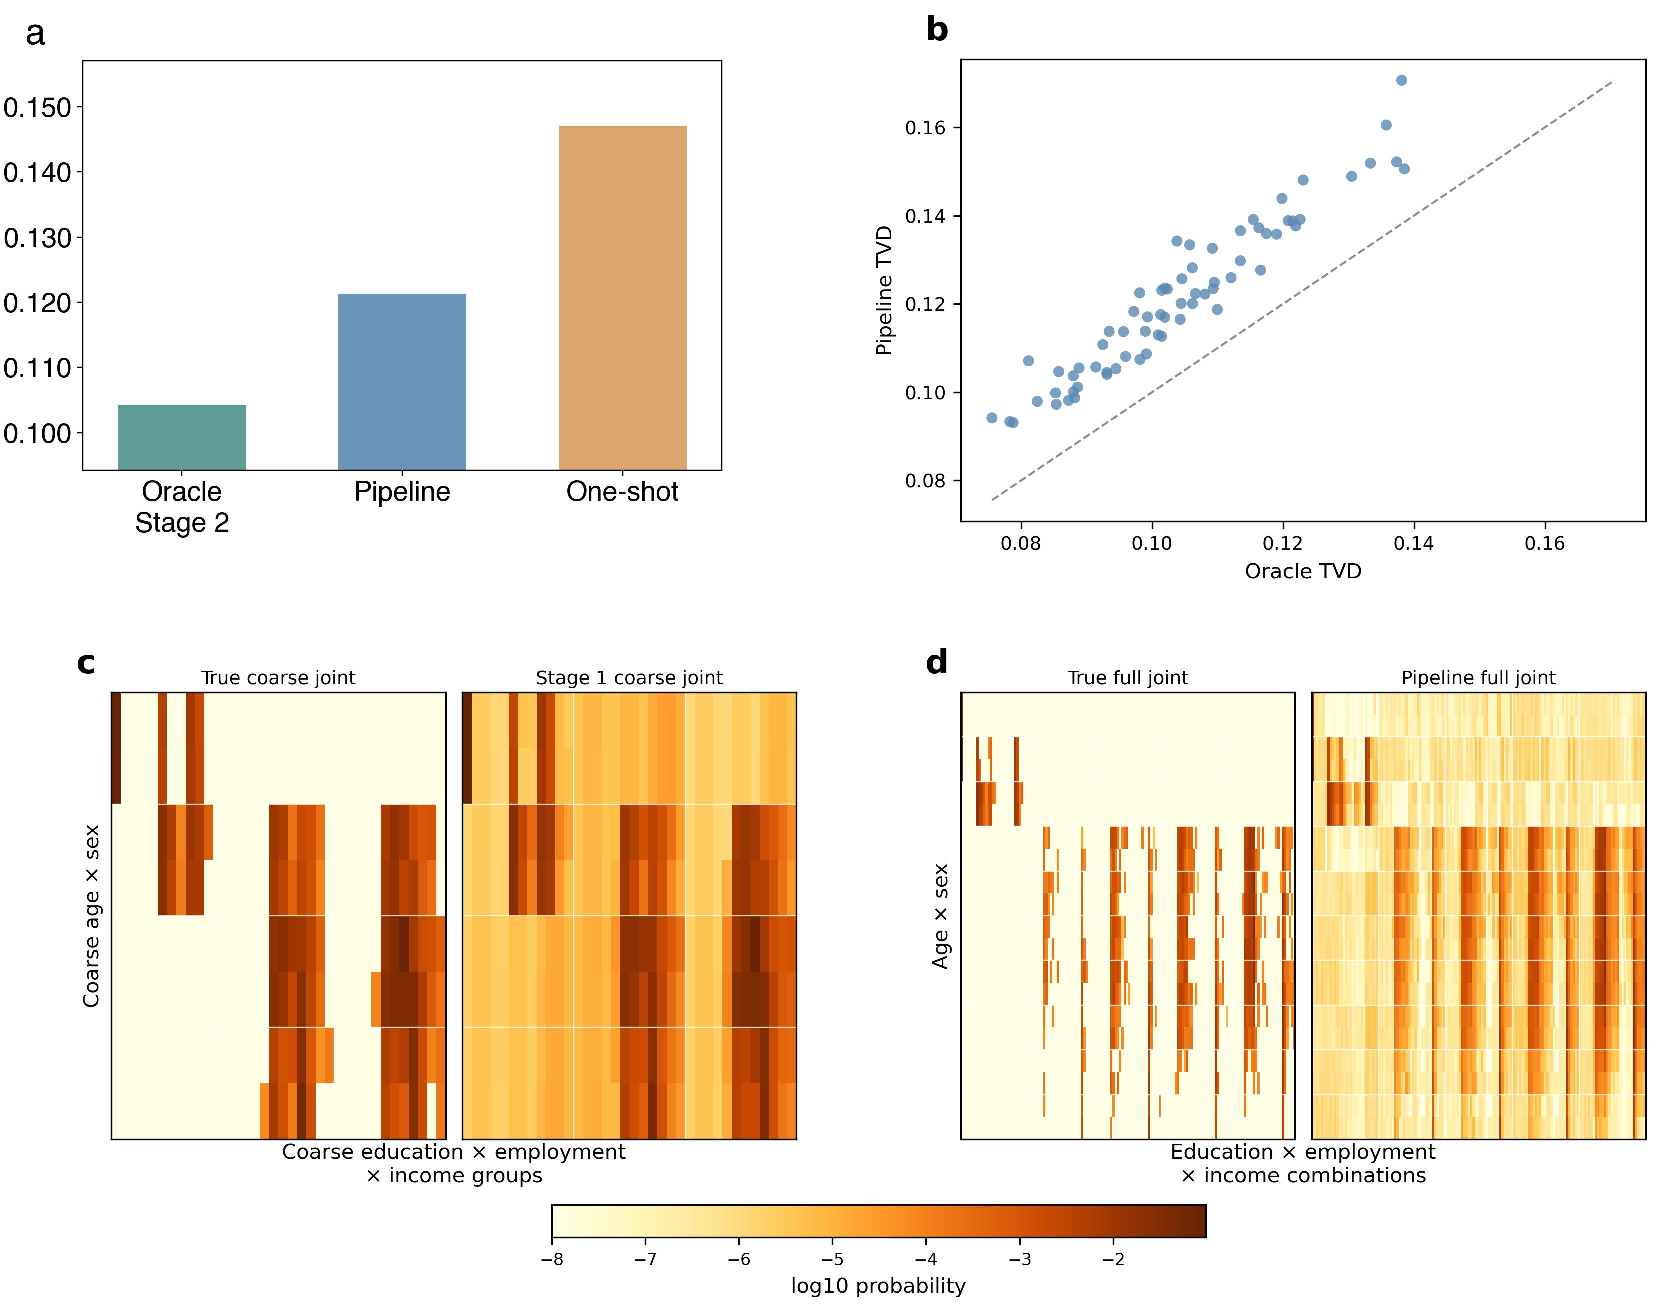
\includegraphics[width=\textwidth]{figures/fig_07_hierarchical_recovery.pdf}
\caption{Hierarchical recovery of the joint distribution on Michigan PUMAs excluded from training. Panel a reports the mean TVD of oracle Stage~2, the hierarchical model, and the one-shot model across three seeds. Panel b compares the per-PUMA TVD of the hierarchical model with oracle Stage~2 TVD; points above the dashed line indicate error inherited from Stage~1. Panels c and d show a representative Michigan PUMA. Panel c compares the true and Stage~1 coarse joints, and panel d compares the true joint distribution with the distribution recovered by the hierarchical model.}
\label{fig:hierarchical_recovery}
\end{figure}

\FloatBarrier


\section{Discussion}

The Michigan experiments show that public census summaries contain enough information to recover a substantial part of the region-specific joint distribution. The pairwise decomposition clarifies where this information enters. Age and sex are already jointly constrained by B01001, so the gain over IPF is small for that pair. Larger gains appear in pairs such as education--employment and education--income, whose dependence must be inferred from regional structure. The stage-wise analysis then shows why the hierarchical model helps. It first recovers broad regional organization at a coarser level and then refines that structure into the joint distribution. A single flat model would need to learn both tasks simultaneously.

This regional result matters because the target product is spatial. Once the recovered joint distribution is converted into explicit home and work locations, the residential layer remains well aligned with the external mobility reference at both tract and within-tract scales, and the work layer captures the main geography of workplace destinations together with the overall commute scale. The framework therefore does more than reconstruct a regional table. It yields a spatially explicit population whose main residential and workplace patterns remain interpretable after location assignment.

The clearest limitation lies on the work side. Home assignment is anchored by residential mass and local residential ordering. Work assignment must also resolve who works, where workers travel, and where they are placed locally within destination tracts. This additional structure makes workplace generation harder than home generation. A second limitation concerns the information carried by the available public summaries. The current income dimension is tied to B20001 and PERNP, and Supplementary Figure~\ref{fig:S1_scaling} shows that finer state spaces quickly outgrow that information.

These results suggest that future progress will depend less on enlarging a flat generator and more on strengthening the information available at the stages where uncertainty remains highest. Richer census summaries can improve dependence recovery, and stronger workplace signals can improve destination assignment. For applications that must build spatially explicit populations from public census summaries, the more promising direction is to match the model decomposition to the structure of the observable information.

%% ====================================================================
\FloatBarrier
\section{Data availability}
The underlying data are ACS PUMS public-use files, available from the United States Census Bureau. Processed joint probability tables and experiment outputs are archived in the project repository.

\section{Code availability}
All scripts for data processing, model training, sampling, and evaluation are available in the project repository.

\bibliographystyle{unsrt}
\bibliography{references}

%% ====================================================================
\clearpage
\appendix
\section*{Supplementary Information}

\subsection*{S1. Dimensional scaling and the information-sparsity boundary}

All five configurations with $K\leq256$ show diffusion advantage over IPF. Testing whether this holds at higher dimensionality, we train on $K=512$ (fine-grained 5-variable joint: $4\times2\times4\times4\times4$ bins). Diffusion TVD reaches 0.139 while IPF achieves 0.112, a reversal of $+0.028$ (Supplementary Table~S1).

Two mechanisms drive this reversal. First, \textit{cell sparsity}: at $K=32$, each joint cell contains $\sim$220 persons on average; at $K=512$, only $\sim$14, making empirical probability estimates unreliable as training targets. Second, \textit{constraint insufficiency}: the pairwise condition vector provides 128 parameters, but the $K=512$ joint has 511 free parameters---a coverage ratio of 25\%, versus 129\% at $K=32$. Extending training from 10k to 30k epochs reduces TVD from 0.182 to 0.147 ($-$19\%) but does not reach IPF's 0.112, confirming the bottleneck is information, not optimization. A counterintuitive corollary: pairwise conditioning at $K=512$ (TVD = 0.249) is \textit{worse} than marginal-only (0.147), because the 128-dim pairwise input must reconstruct 511 unknowns without the global-prior support that IPF supplies to the marginal-only pipeline.

\begin{table}[htbp]
\centering
\caption{Supplementary Table S1. Dimensional scaling comparison between diffusion and IPF.}
\label{tab:S1_Kscale}
\begin{tabular}{ccccc}
\toprule
$K$ & Variables & Diff.\ TVD & IPF TVD & $\Delta$ \\
\midrule
32  & 5-var & 0.024 & 0.058 & $-0.034$ \\
64  & 2-var & 0.069 & 0.074 & $-0.005$ \\
64  & 3-var & 0.055 & 0.070 & $-0.015$ \\
128 & 5-var & 0.051 & 0.081 & $-0.030$ \\
256 & 3-var & 0.084 & 0.103 & $-0.019$ \\
512 & 5-var & 0.139 & 0.112 & $+0.028$ \\
\bottomrule
\end{tabular}
\vspace{2pt}
\begin{minipage}{0.98\linewidth}
\footnotesize
\textit{Notes:} $\Delta = \text{Diffusion TVD} - \text{IPF TVD}$ (negative is better for diffusion). For each $K$, the diffusion entry reports the best available condition setting under the corresponding experiment protocol.
\end{minipage}
\end{table}

\begin{figure}[htbp]
\centering
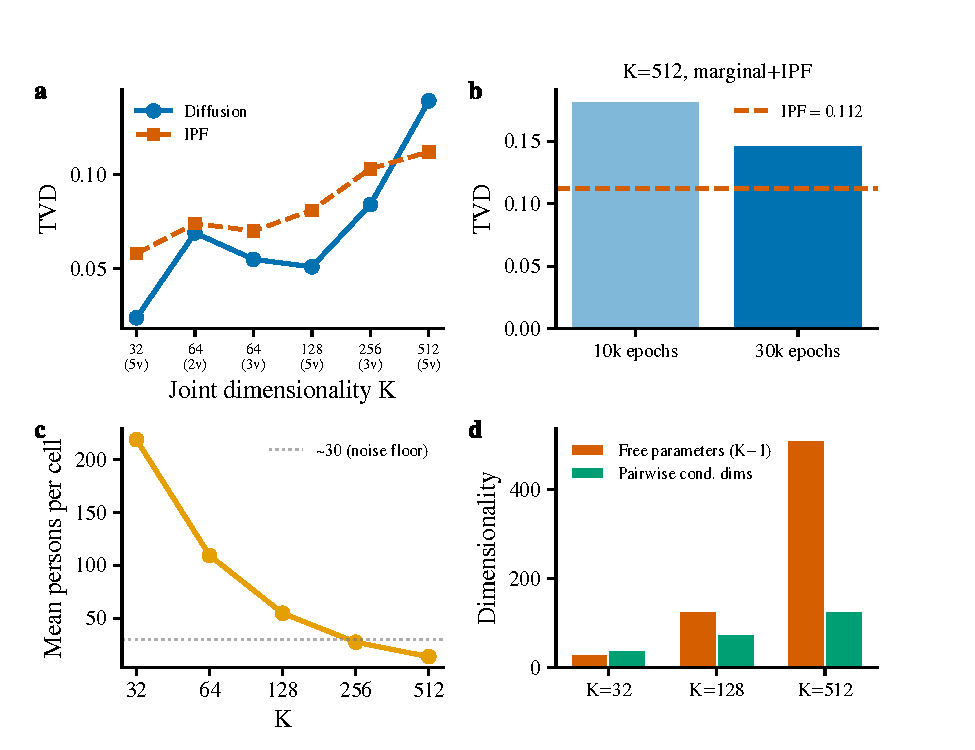
\includegraphics[width=\textwidth]{figures/fig_s01_scaling.pdf}
\caption{\textbf{Supplementary Fig.~S1.} Dimensional scaling and information boundaries.
(a)~Diffusion TVD and IPF TVD vs.\ joint dimensionality $K$. Crossover near $K\approx 400$.
(b)~Training effect at $K=512$: TVD at 10k and 30k epochs, with IPF reference.
(c)~Average persons per cell vs.\ $K$, illustrating sparsity growth.
(d)~Constraint coverage: pairwise condition dimensions vs.\ joint free parameters.}
\label{fig:S1_scaling}
\end{figure}

\begin{figure}[htbp]
\centering
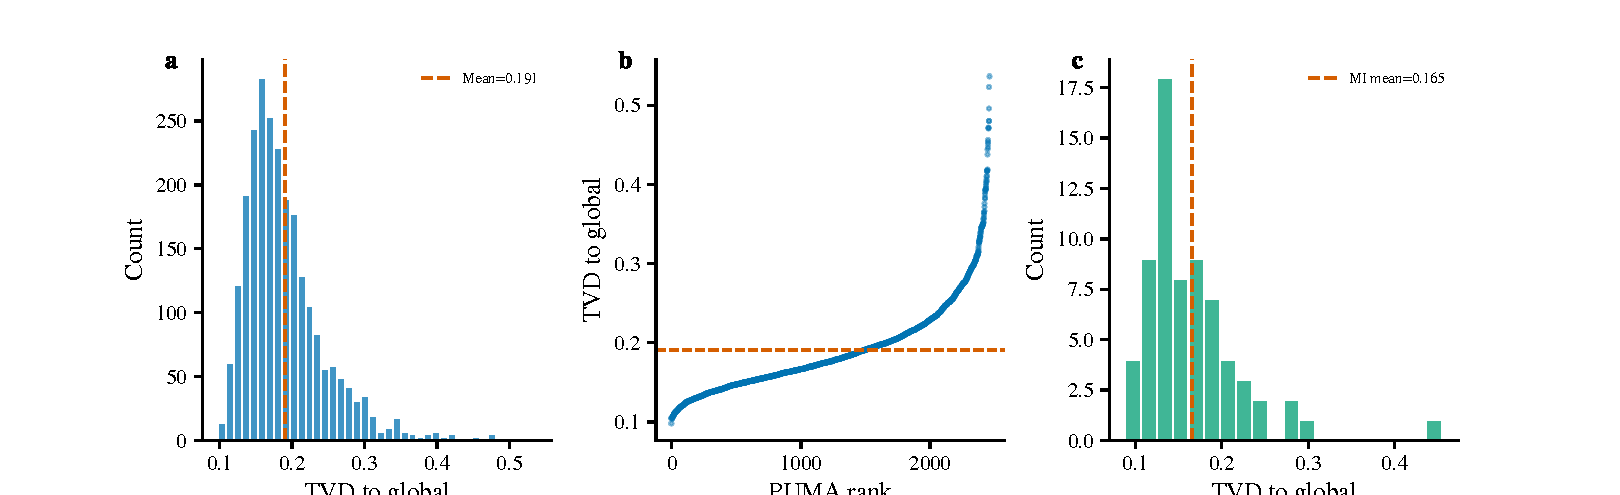
\includegraphics[width=\textwidth]{figures/fig_s02_heterogeneity_stats.pdf}
\caption{\textbf{Supplementary Fig.~S2.} Distribution of dependence heterogeneity.
(a)~Histogram of TVD-to-global for 2,456 regions in the United States. Mean = 0.191 (dashed); 90th percentile = 0.265.
(b)~Rank-ordered TVD across all regions; the long right tail shows a substantial minority deviate strongly from the national average.
(c)~Same metric for Michigan's 68 regions (the held-out test state), showing that Michigan spans a representative range of heterogeneity levels.}
\label{fig:S2_heterogeneity}
\end{figure}

\begin{figure}[htbp]
\centering
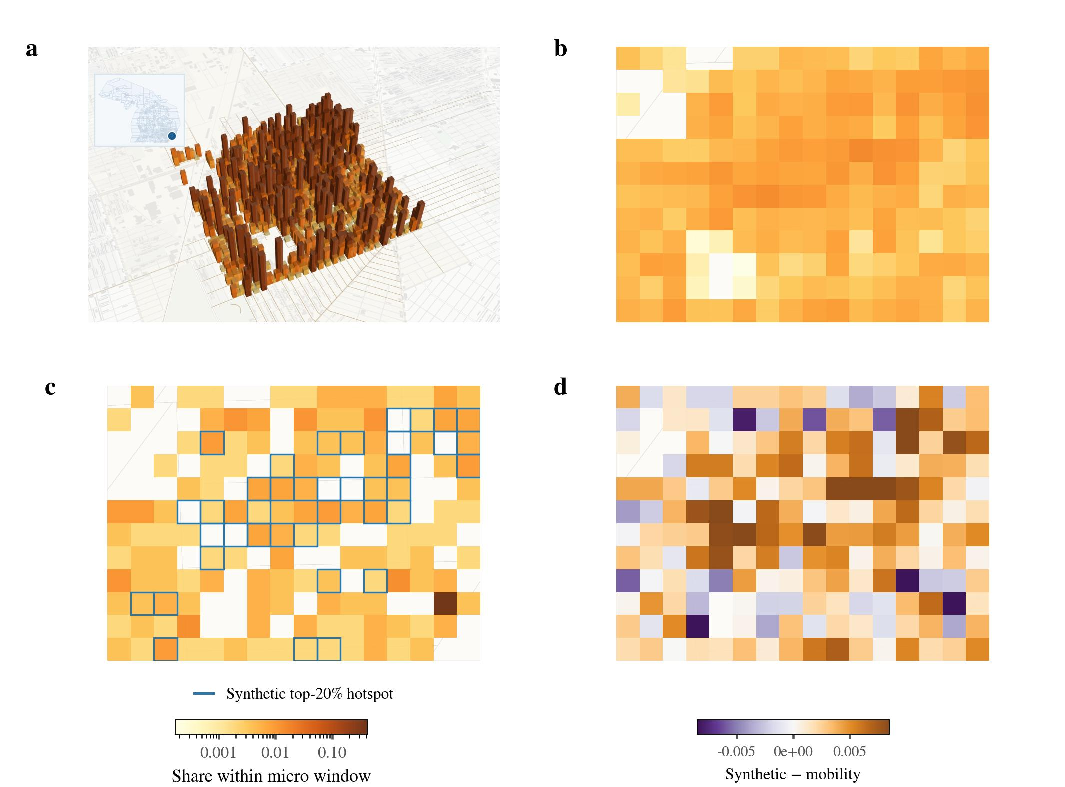
\includegraphics[width=\textwidth]{figures/fig_s03_home_micro_validation.pdf}
\caption{\textbf{Supplementary Fig.~S3.} Local residential validation in a Detroit micro-window.
(a)~Synthetic home-point density rendered in a local three-dimensional view.
(b)~Synthetic residential share across the micro-window.
(c)~Synthetic top-20\% hotspots overlaid on the same local grid.
(d)~Difference between the synthetic and mobility-derived residential shares in the same micro-window.}
\label{fig:S3_home_micro}
\end{figure}

\end{document}
